\section{Introduzione}

\subsection{Glossario}
In questo documento sono state segnate con il pedice "g" tutte le parole che, secondo noi, necessitano di una spiegazione ulteriore per evitare
eventuali ambiguità o incomprensioni.

La spiegazione di questi termini la si può trovare nel documento di \textit{Glossario}.

\subsection{Scopo del documento}
Il documento \textit{Specifica Tecnica} ha lo scopo di descrivere i componenti utilizzati e le scelte progettuali fatte per la realizzazione del prodotto.

Dopo aver fornito un elenco descrittivo dei componenti verranno spiegati nel dettaglio, utilizzando l'ausilio degli schemi UML, i seguenti punti di interesse: 
\begin{itemize}
	\item Design pattern architetturale determinato dalle tecnologie adottate;
	\item Architettura logica (dipendenze e interazioni tra componenti);
	\item Architettura di deployment;
	\item Altri aspetti progettuali.
\end{itemize}

\subsection{Suggerimenti per la comprensione del documento}
Per comprendere al meglio l'architettura utilizzata è importante comprendere in primo luogo il design pattern
architetturale derterminato dalle tecnologie adottate in quanto gran parte delle scelte fatte si basano su di esso.

\textbf{Si suggerisce quindi di leggere la sezione} \ref{design Redux} \textbf{riguardante il design pattern architetturale determinato 
dalle tecnologie adottate prima di proseguire con le successive}.

\subsection{Riferimenti}
\subsubsection{Riferimenti normativi}
\begin{itemize}
\item .
\end{itemize}

\subsubsection{Riferimenti informativi}
\begin{itemize}
\item .
\end{itemize} 

\section{Descrizione dell'architettura}
\subsection{Elenco dei componenti}
\begin{itemize}
	\item \textbf{\large Slices}
	\\\\
	Le Slice contengono una porzione dello stato globale dell'applicazione che è gestita da un reducer specifico.
		\begin{itemize}
			\item \textbf{CartSlice}: componente che permette la gestione dello stato che contiene i dati riguardanti il carrello;
			\item \textbf{ProductsSlice}: componente che permette la gestione dello stato che contiene i dati riguardanti i prodotti 
			presenti all'interno dell'ambiente 3D;
			\item \textbf{PlayerSlice}: componente che permette la gestione dello stato che contiene i dati riguardanti il player;
			\item \textbf{RayCasterSlice}: componente che permette la gestione dello stato che contiene i dati riguardanti il
			raycaster;
			\item \textbf{DecorationSlice}: componente che permette la gestione dello stato che contiene i dati riguardanti
			il caricamento delle decorazioni all'interno dell'ambiente 3D;
			\item \textbf{SidebarSlice}: componente che permette la gestione dello stato che contiene i dati riguardanti
			la side-bar.
		\end{itemize}
	\item \textbf{\large Initial states}
	\\\\
	Gli stati iniziali risiedono all'interno di ciascuna slice e la loro unione contiene i dati che formano lo stato globale dell'applicazione gestito dallo store.
	Tutti gli altri dati sono contenuti e gestiti dai componenti React che li utilizzano.
		\begin{itemize}
			\item \textbf{CartInitialState}: componente che contiene i dati relativi agli oggetti presenti all'interno del carrello;
			\item \textbf{ProductsInitialState}: componente che contiene i dati relativi ai prodotti presenti all'interno dell'ambiente 3D;
			\item \textbf{PlayerInitialState}: componente che contiene i dati relativi al player;
			\item \textbf{RayCasterInitialState}: componente che contiene i dati utili ad interagire con un oggetto presente all'interno dell'
			ambiente 3D;
			\item \textbf{DecorationInitialState}: componente che contiene la lista di tutte le decorazioni presenti all'interno dell'ambiente 3D;
			\item \textbf{SidebarInitialState}: componente che contiene i dati utili a reperire informazioni sulla sidebar;
		\end{itemize}
		\item \textbf{\large Actions}
		\\\\
		Le azioni sono emesse dai componenti e sono inviate ai reducers per aggiornare lo stato corrispondente.
		Le azioni sono caratterizzate da un type e da un payload che viene utilizzato dalle slice per modificare lo stato.
		\\
		Per convenzione il nome delle azioni segue il formato: [nome Slice dalla quale viene catturata].[nome azione].
		\begin{itemize}
			\item \textbf{sidebar.toggleSidebarIsOpen}: azione emessa quando si apre o si chiude la sidebar relativa ad un prodotto presente 
			all'interno della scena 3D.
			\\
			Payload: nessuno;
			\item \textbf{products.setSelectedColor}: azione emessa quando si seleziona nella sidebar un nuovo colore per un prodotto.
			\\
			Payload: PayloadSetSelectedColor \{id:number, selectedColor: String\};
			\\
			id: ID del prodotto a cui cambiare il colore.
			\\
			selectedColor: colore selezionato;
			\item \textbf{rayCaster.setLastProductPointed}: azione emessa per aggiornare l'ID che rappresenta l'ultimo oggetto puntato dal raycaster.
			\\
			Payload: \{id:number\}
			\\
			id: ID dell'ultimo prodotto puntato dal raycaster;
			\item \textbf{rayCaster.toggleRayCasterEnabled}: azione emessa per abilitare o disabilitare il raycaster.
			\\
			Payload: nessuno;
			\item \textbf{cart.addItems}: azione emessa per aggiungere uno o più prodotti al carrello.
			\\
			Payload: PayloadAddItems \{id: number, price: number, quantity: number,selectedColor: String\}
			\\
			id: ID del prodotto da aggiungere al carrello.
			\\
			price: prezzo del prodotto da aggiungere al carrello.
			\\
			quantity: quantità di prodotti da aggiungere al carrello.
			\\
			selectedColor: colore selezionato del prodotto da aggiungere al carrello.
			\item \textbf{cart.removeItem}: azione emessa per rimuovere un prodotto dal carrello.
			\\
			Payload: \{id:number\}
			\\
			id: ID del prodotto da rimuovere al carrello.
			\item \textbf{cart.removeAll}: azione emessa per rimuovere tutti i prodotti presenti nel carrello.
			\\
			Payload: nessuno;
		\end{itemize}
		\item \textbf{\large Model components}
		\\\\
		Classi offerte dalle librerie utilizzate:
		\begin{itemize}
			
			\item \textbf{Camera}: classe offerta dalla libreria three.js.
			Rappresenta l'utente all'interno dell'ambiente 3D.
			Modificando gli attributi di questa classe l'utente compie movimenti spaziali e può esplorare l'ambiente che 
			lo circonda da prospettive diverse;
			\item \textbf{Octree}: classe offerta dalla libreria three.js.
			L'Octree è una struttura dati ad albero utilizzata per la rappresentazione e la gestione di dati spaziali 
			tridimensionali. 
			In particolare, viene utilizzata per dividere lo spazio tridimensionale in regioni più piccole, 
			suddividendo ciascuna regione in otto sotto-regioni.
			Utile per determinare con quale prodotto si sta interagendo o per rilevare le collisioni;
			\item \textbf{Vector3}: classe offerta dalla libreria three.js.
			Rappresenta un vettore tridimensionale, ovvero una grandezza fisica caratterizzata da una direzione e da una lunghezza.
			Il vettore tridimensionale viene comunemente utilizzato per definire la posizione, la rotazione, 
			la scala e la direzione degli oggetti all'interno di una scena 3D;
			\item \textbf{Capsule}: classe offerta dalla libreria three.js.
			La classe Capsule offre la possibilità di impostare una forma di collisione personalizzata 
			per l'oggetto rappresentato dalla capsula; 
			\item \textbf{Store}: Lo store in Redux è l'oggetto che tiene traccia dello stato dell'applicazione. 
			Contiene il reducer che specifica come le azioni influenzano lo stato e offre metodi per accedere allo stato corrente, 
			inviare azioni e registrare funzioni di callback per essere avvisati quando lo stato cambia;
			\item \textbf{RootReducer}: componente Redux che combina tutti i reducers dell'applicazione in uno stato globale. 
			Questa funzione viene passata allo store per gestire lo stato complessivo dell'applicazione.
		\end{itemize}
		Classi definite dall'utente:
		\begin{itemize}
			\item \textbf{CartItem}: classe che rappresenta un item all'interno del carrello.
			Quando viene aggiunto un prodotto al carrello viene creato un item che ne raccoglie le informazioni utili 
			alla sua visualizzazione all'interno del carrello e all'acquisto;
			\item \textbf{Product}: classe che rappresenta un prodotto acquistabile dall'utente;
			\item \textbf{ModelGLTF}: classe che rappresenta il modello 3D di un prodotto acquistabile da caricare all'interno della scena;
			\item \textbf{PayloadAddItems}: classe che rappresenta il payload da passare ad una AddItems action;
			\item \textbf{Decoration}: classe che rappresenta una decorazione all'interno della scena;
			\item \textbf{DecorationModelGLTF}: classe che rappresenta il modello 3D di una decorazione da caricare all'interno della scena;
			\item \textbf{PayloadSetSelectedColor}: classe che rappresenta il payload da passare ad una SetSelectedColor action;
			\item \textbf{Color}: classe che rappresenta un colore che può essere associato ad un ModelGLTF; 
			\item \textbf{Coordinate}: classe utilizzata per indicare un punto all'interno dell'ambiente 3D;
			\item \textbf{Player}: classe con il compito di tenere traccia ed aggiornare le informazioni riguardanti 
			lo stato dell'utente all'interno dell'ambiente 3D.
			Le informazioni principali di cui si occupa sono la posizione spaziale, la posizione della camera e
			la velocità con cui l'utente si muove.
		\end{itemize}
		
		\item \textbf{\large UI React components}
		\\\\
		I seguenti componenti hanno il compito di visualizzare i dati dello stato che costituiscono l'interfaccia 
		utente. 
		\begin{itemize}
			\item \textbf{UI}: contiene i componenti grafici che vanno a costituire l'interfaccia
			utente; 
			\item \textbf{Crosshair}: componente react-three-fiber che viene utilizzato per aiutare l'utente a puntare
			un determinato punto nello spazio 3D.
			Viene indicato con un punto o una croce al centro dello schermo ed usato come puntatore dall'utente;
			\item \textbf{Cart}: rappresenta il carrello;
			\item \textbf{CartItem}: rappresenta un prodotto all'interno del carrello.
			Contiene le informazioni necessarie alla visualizzazione e all'acquisto di un prodotto;
			\item \textbf{ProductUI}: contiene i componenti dell'interfaccia utente per la visualizzazione
			del ProductInteractionPrompt e della sidebar;
			\item \textbf{Sidebar}: contiene i componenti necessari a visualizzare i 
			dettagli del prodotto con cui si sta iteragendo e i componenti con cui è possibile modificare le caratteristiche del 
			prodotto e aggiungerne la quantità specificata al carrello;
			\item \textbf{ColorSelector}: contiene i componenti necessari per compiere un'azione di selezione colore;
			\item \textbf{SelectColorItem}: componente con cui è possibile compiere un'azione di selezione colore;
			\item \textbf{ProductDetails}: componente per la visualizzazione dei dettagli di un prodotto;
		\end{itemize}
		\item \textbf{\large 3D React components}
		I seguenti componenti hanno il compito di visualizzare i dati dello stato contenuti all'interno del canvas 
		sul quale viene renderizzata la scena 3D.
		\begin{itemize}
			\item \textbf{Provider}: Il Provider nel contesto Redux è un componente che consente di rendere lo store accessibile
			a tutti i componenti dell'applicazione. 
			Viene 'avvolto' intorno al componente principale dell'applicazione App e accetta lo store come prop; 
			\item \textbf{App}: componente radice dell'applicazione che contiene tutti gli altri componenti. 
			È 'avvolto' dal Provider di Redux per fornire accesso allo store a tutti i componenti figli;
			\item \textbf{Canvas}: componente react-three-fiber che comprende gli elementi grafici che vanno a costituire
			la scena 3D.
			Canvas si occupa di creare un nuovo canvas HTML e di associarlo a una nuova istanza di THREE.WebGLRenderer, 
			che viene utilizzata per renderizzare la scena.
			Fornisce una camera e una scena con una serie di props opzionali utili alla configurazione dell'ambiente 3D;
			\item \textbf{Scene}: componente react-three-fiber che rappresente l'ambiente 3D.
			Si tratta di uno spazio virtuale 3D in cui gli oggetti vengono posizionati, orientati e illuminati; 
			\item \textbf{PointerLock}: componente react-three-fiber che consente di "bloccare" il puntatore del mouse all'interno 
			di un elemento specifico della pagina web.
			Permette quindi di controllare la camera e di disattivarne i controlli quando 
			necessario (ad esempio quando si apre un menu di interazione con un prodotto);
			\item \textbf{Environment}: componente react-three-fiber utilizzato per creare un'ambientazione configurata
			secondo impostazioni standard settabili;
			\item \textbf{Map}: contiene i componenti che costituiscono la scena.
			\item \textbf{FlashLight}: rappresenta una luce direzionale utilizzata dall'utente per illuminare
			l'ambiente 3D;
			\item \textbf{Player}: rappresenta l'utente all'interno dell'ambiente 3D;
			\item \textbf{Lights}: rappresenta le luci all'interno della scena;
			\item \textbf{Model}: rappresenta un prodotto all'interno dell'ambiente 3D;
			I modelli vengono caricati all'interno della scena specificandone il path del modello .gltf, la posizione
			in cui si vogliono collocare e le caratteristiche del prodotto legato al modello;
			\item \textbf{Decorations}: modello .gltf che si differisce dal modello di un prodotto 
			per il fatto che non è modificabile e con il quale non si può interagire;
			\item \textbf{RayCaster}: 
			il raycaster genera un raggio virtuale che parte dalla posizione del puntatore del mouse e attraversa lo schermo fino a 
			raggiungere un oggetto nella scena, se presente. 
			È possibile quindi utilizzare questa informazione per eseguire azioni in risposta all'interazione dell'utente.
		\end{itemize}
\end{itemize}
\subsection{Design pattern architetturale determinato dalle tecnologie adottate}
\label{design Redux}

\subsubsection{Redux-Toolkit}
I componenti che costituiscono l'architettura utilizzata seguono il pattern offerto dalla libreria Redux-Toolkit.

Redux-Toolkit è pensato per integrarsi con React e il principale vantaggio che offre è quello di poter gestire i dati condivisi tra 
i componenti React in modo centralizzato semplificando la gestione dello stato globale dell'applicazione.
\\\\
I componenti che formano l'architettura di Redux-Toolkit sono:
\begin{itemize}
	\item \textbf{Store}: componente che contiene lo stato globale dell'applicazione.
	
	All'avvio dell'applicazione viene configurato utilizzando RootReducer e i componenti che utilizzano lo stato globale fanno il subscribe allo \textit{store}
	in modo da venire renderizzati ogni volta che un dato di interesse cambia valore.
	Questo modo di operare può essere visto come un pattern \textit{Observer} in cui lo \textit{store} è il \textit{Subject} e gli \textit{Observers} sono i componenti React che hanno fatto 
	il subscribe allo \textit{store};
	\item \textbf{RootReducer}: componente utilizzato per configurare lo store combinando le slice;
	\item \textbf{Slice}: componente che contiene un proprio stato che rappresenta una porzione dello stato globale dell'applicazione, i \textit{reducer}
	che operano su tale stato e i \textit{selector} per consentire ai suoi client il reperimento dei dati. 

	Per definire una \textit{slice} è buona norma raggruppare i dati in modo che siano legati da un sottoinsieme di funzionalità offerte dal sistema che lavorano 
	su dati comuni;  
	\item \textbf{Reducer}: componente che riceve come parametri uno stato iniziale (\textit{InitialState}) e una \textit{action} (composta da un type e un payload) e restituisce 
	lo stato dopo aver operato sui dati. 
	
	React-Toolkit gestisce le chiamate ai \textit{reducer} in seguito ai dispatch delle \textit{action} che avvengono
	specificando solamente l'oggetto che rappresenta il payload;
	\item \textbf{Actions}: oggetto composto da un type e da un payload di cui viene effettuato il dispatch quando opportuno. 
	
	Il payload è un oggetto che contiene i dati da passare al \textit{reducer} che catturerà l'\textit{action};
	\item \textbf{InitialState}: componente che contiene i dati di una \textit{slice} su cui essa opera. 
	
	Importante precisare che Redux-Toolkit utilizzando 
	la libreria immer gestisce anche l'immutabilità dei dati in modo che i reducer restituiscano delle copie dello stato in modo che esso non possa 
	venire modificato dall'esterno e utilizzato in modo improrio.
	
	L'unico modo per modificare i dati dello stato globale è quindi con il dispatch di un'\textit{action};
	\item \textbf{Selector}: funzione che prende lo stato corrente di una \textit{slice} come argomento e ritorna un sottoinsieme specifico
	del suo stato. In altre parole, un \textit{selector} consente di 'selezionare' una parte specifica dello stato
	in modo da poterla utilizzare in modo isolato all'interno di un componente React.
\end{itemize}

\subsubsection{React-three-fiber}
Questa libreria fornisce un 'punto d'incontro' tra React (libreria javascript per la creazione di interfacce utente) e Three.js (libreria usata per
la modellazione dell'ambiente 3D) semplificando la creazione dei componenti da inserire all'interno dell'ambiente 3D.

React-three-fiber rende la scrittura del codice dichiarativa creando dei componenti React 'preconfezionati' che rappresentano i componenti 3D.
Questi componenti sono personalizzabili modificandone le caratteristiche tramite le props di React.

Un esempio è il componente \textit{Canvas} che fornisce con un'unica dichiarazione la \textit{scene} e la \textit{camera} con una configurazione standard 
adatta alla maggior parte dei casi di utilizzo. Per inserire i componenti all'interno dell'ambiente è sufficiente dichiararli come figli del 
componente \textit{scene}.
\subsection{Architettura logica}
Per facilitare la lettura dei diagrammi delle classi è stato scelto di organizzarli per feature in modo che ogni diagramma 
rappresenti i componenti che permettono l'implementazione di funzionalità specifiche.
Sono presenti dei diagrammi che non seguono questa convenzione che sono utili per avere una visione generale sulle dipendenze
di alcuni componenti.
\\\\
I diagrammi prodotti che rappresentano funzionalità specifiche sono:
\begin{itemize}
	\item \textbf{CartFeaturesDiagram}: include i componenti che svolgono le funzioni riguardanti il carrello;
	\item \textbf{PlayerFeaturesDiagram}: include i componenti che svolgono le funzioni riguardanti le interazioni dell'utente con 
	l'ambiente 3D;
	\item \textbf{SidebarFeaturesDiagram}: include i componenti che svolgono le funzioni riguardanti la side-bar;
	\item \textbf{InterfaceFeaturesDiagram}: include i componenti necessari per il corretto aggiornamento dell'interfaccia utente.
\end{itemize}
I diagrammi prodotti che forniscono una visione generale delle dipendenze tra componenti sono:
\begin{itemize}
	\item \textbf{StoreDiagram}: include lo \textit{store} e le slice che compongono lo stato globale dell'applicazione;
	\item \textbf{SkyLevelReactComponentsHierarchy}: contiene i macrocomponenti React che costituiscono l'applicazione;
	\item \textbf{UIReactComponentsHierarchy}: contiene i componenti che costituiscono l'interfaccia utente;
	\item \textbf{CanvasReactComponentsHierarchy}: contiene i componenti che costituiscono gli elementi dell'ambiente 3D.
\end{itemize}
\newgeometry{margin=0.5cm}
\begin{landscape}
	\thispagestyle{empty}
	\subsubsection{CartFeaturesDiagram}
	\begin{figure}[H]
		\centering
		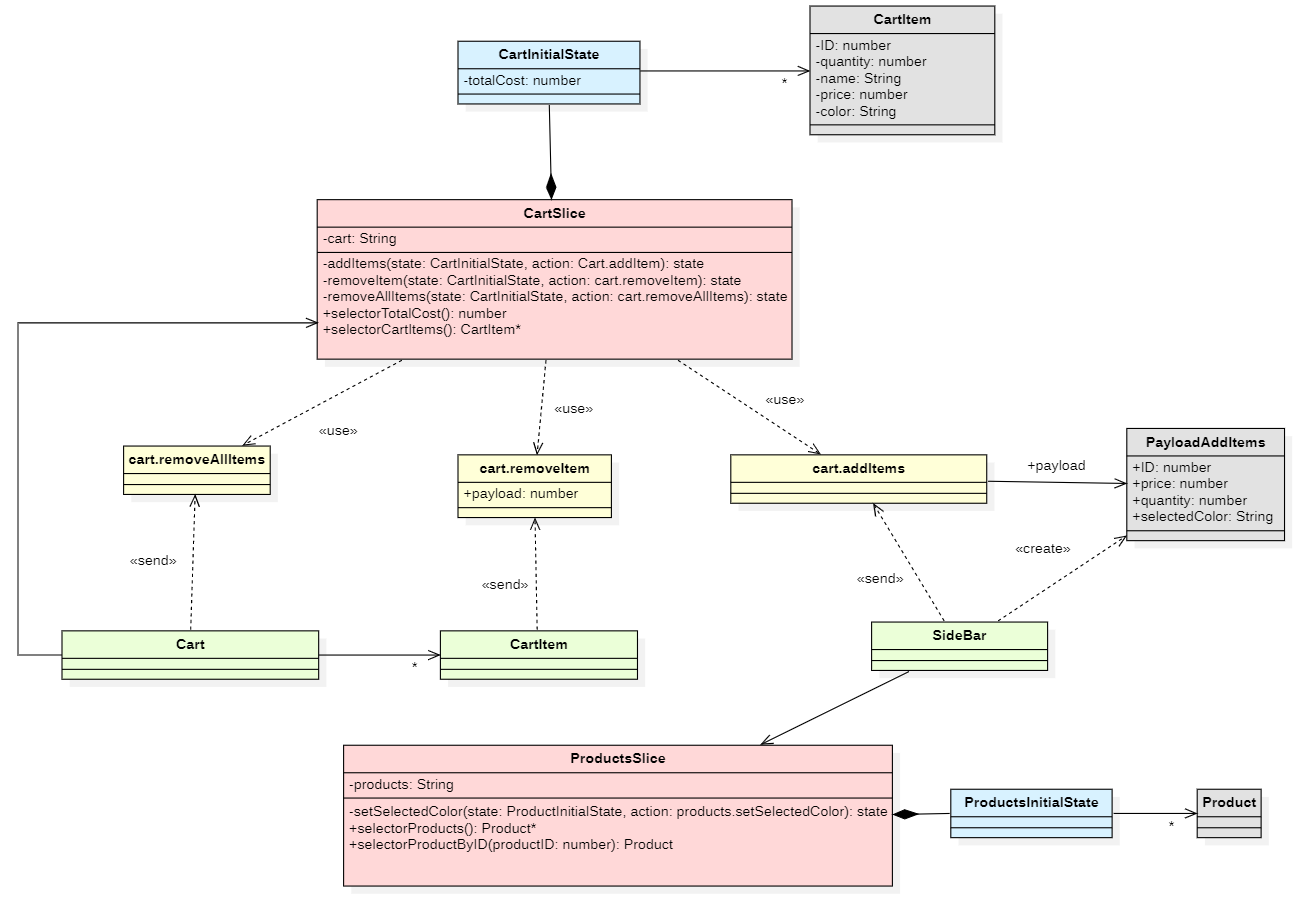
\includegraphics[scale=0.75, keepaspectratio]{./res/images/CartFeaturesDiagram.PNG}
		\caption[UML delle classi CartFeaturesDiagram]{
		UML delle classi CartFeaturesDiagram.
		\\
		\textbf{Legenda}: 
		[\textit{Slices}: rosso] -
		[\textit{Actions}: giallo] -
		[\textit{Model classes}: grigio] -
		[\textit{Initial states}: azzurro] -
		[\textit{UI React components}: verde]}
	\end{figure}
\end{landscape}
\restoregeometry

\paragraph*{Descrizione del diagramma:}
CartFeaturesDiagram include i componenti che svolgono le funzioni riguardanti il carrello.
\begin{itemize}
		\item \textbf{CartSlice}
		\\\\
		\textbf{Dipendenze}:
		\begin{itemize}
			\item \textit{CartInitialState} (composizione): si occupa della costruzione e distruzione dell'istanza di CartInitialState
			che non viene condivisa con altri componenti in quanto CartSlice si occupa in modo esclusivo della sua gestione.
			\item \textit{CartItem} (dipendenza semplice \textless create\textgreater): si occupa della costruzione dei CartItem 
			da inserire all'interno della lista items di CartInitialState;
			\item \textit{cart.addItems} (Dipendenza semplice \textless use\textgreater): cattura un'istanza di cart.addItems e il 
			reducer ne utilizza il payload per aggiungere un item ad items in CartInitialState.
			Se le caratteristiche specificate nel payload corrispondono a quelle di un item presente ne incrementa la quantità 
			del valore specificato altrimenti viene aggiunto un nuovo item con le caratteristiche e quantità specificate;  
			\item \textit{cart.removeItem} (Dipendenza semplice \textless use\textgreater): cattura un'istanza di cart.removeItem e il reducer
			ne utilizza il payload per decrementare la quantità dell'item specificato.
			Se la quantità dopo il decremento risulta essere uguale a 0 l'item viene rimosso da items in CartInitialState;
			\item \textit{cart.removeAllItems} (Dipendenza semplice \textless use\textgreater): cattura un'istanza di cart.removeAllItems e chiama il reducer 
			che svuota la lista items presente in CartInitialState ed imposta il totalCost a 0.
		\end{itemize}
		\textbf{Interazioni}:
		\begin{itemize}
			\item \textit{CartInitialState}: viene modificato in base alle actions catturate dal reducer della slice.
		\end{itemize}
		\textbf{Actions catturate}:
		\begin{itemize}
			\item \textit{cart.addItems}: utilizzata dal reducer per chiamare \textit{addItems};
			\item \textit{cart.removeItem}: utilizzata dal reducer per chiamare \textit{removeItem};
			\item \textit{cart.removeAllItems}: utilizzata dal reducer per chiamare \textit{removeAllItems}.
		\end{itemize}
		\item \textbf{CartInitialState}
		\\\\
		\textbf{Dipendenze}: 
		\begin{itemize}
			\item \textit{CartItem} (Associazione): contiene la lista degli item che rappresentano i prodotti presenti nel carrello.
		\end{itemize} 
		\item \textbf{Cart}
		\\\\
		\textbf{Dipendenze}:
		\begin{itemize}
		\item \textit{CartItem} (Composizione): crea le istanze di CartItem durante il rendering.
		Cart gestisce interamente il ciclo di vita delle istanze di un CatrItem che quindi per composizione
		non può essere condiviso con altri componenti.
		\item \textit{CartSlice} (Associazione): possiede come attributo implicito (dovuto a Redux) un'istanza di CartSlice.
		\item \textit{cart.removeAllItems} (Dipendenza semplice \textless send\textgreater): crea ed emette un'istanza dell'azione cart.removeAllItems.
	\end{itemize} 
	\textbf{Interazioni}:
	\begin{itemize}
		\item \textit{CartSlice}: chiama i selettori \textit{selectorCartItems} e \textit{selectorTotalCost} per reperire gli items e il costo totale dei prodotti 
		allo scopo di compiere il rendering dei suoi componenti figli.
	\end{itemize}
	\textbf{Action emesse}:
	\begin{itemize}
		\item \textit{cart.removeAllItems}: emessa quando l'utente rimuove tutti i prodotti dal carrello.
	\end{itemize}
	\item \textbf{CartItemReact}
	\\\\
	\textbf{Dipendenze}: 
	\begin{itemize}
		\item \textit{cart.removeItem} (Dipendenza semplice \textless send\textgreater): crea ed emette un'istanza dell'azione cart.removeItem.
	\end{itemize}
	\textbf{Action emesse}:
	\begin{itemize}
		\item \textit{cart.removeItem}: emessa quando l'utente rimuove il prodotto corrispondente all'item dal carrello.
	\end{itemize}
	\item \textbf{Sidebar}
	\\\\
	\textbf{Dipendenze}:
	\begin{itemize}
		\item \textit{ProductsSlice} (Associazione): possiede come attributo implicito (dovuto a Redux) un'istanza di ProductsSlice.
		\item \textit{PayloadAddItems} (Dipendenza semplice \textless create\textgreater): crea il payload da fornire alla action cart.addItems.
		\item \textit{cart.addItems} (Dipendenza semplice \textless send\textgreater): crea ed emette un'istanza dell'azione cart.addItems.
		\end{itemize}
		\textbf{Interazioni}:
		\begin{itemize}
			\item \textit{ProductsSlice}: chiama il selettore \textit{selectorProductByID} per reperire le informazioni del prodotto 
			allo scopo di compiere il rendering dei suoi componenti figli.
		\end{itemize}
\end{itemize}
	
	\newgeometry{margin=0.5cm}
	\begin{landscape}
		\thispagestyle{empty}
		\subsubsection{PlayerFeaturesDiagram}
		\begin{figure}[H]
			\centering
			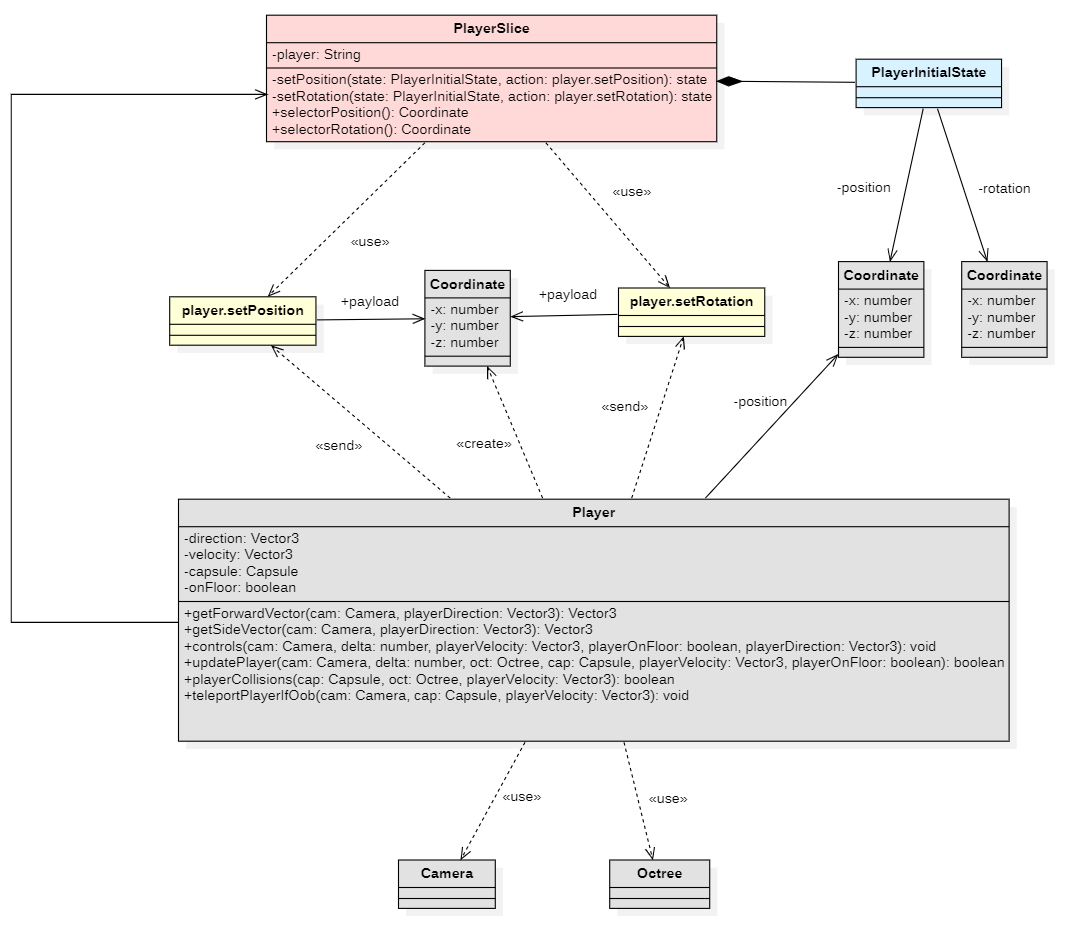
\includegraphics[scale=0.7, keepaspectratio]{./res/images/PlayerFeaturesDiagram.PNG}
			\caption[UML delle classi PlayerFeaturesDiagram]{
				UML delle classi PlayerFeaturesDiagram.
				\\
				\textbf{Legenda}: 
				[\textit{Slices}: rosso] -
				[\textit{Actions}: giallo] -
				[\textit{Model classes}: grigio] -
				[\textit{Initial states}: azzurro] -
				[\textit{UI React components}: verde]}
			\end{figure}
		\end{landscape}
		\restoregeometry
		% Sistemare alcune parti
		\paragraph*{Descrizione del diagramma:}
		PlayerFeaturesDiagram include i componenti che svolgono le funzioni riguardanti le interazioni dell'utente con 
		l'ambiente 3D.
\begin{itemize}
		\item \textbf{Player}
		\\\\
		\textbf{Dipendenze}:
		\begin{itemize}
			\item \textit{Camera} (Dipendenza semplice \textless use\textgreater): utilizza la camera del canvas in cui viene renderizzata l'applicazione
			 per aggiornare la scena 3D;
			\item \textit{Octree} (Dipendenza semplice \textless use\textgreater): usa l'Octree della scena per individuare le collisioni dell'utente con 
			gli oggetti all'interno dell'ambiente 3D.
		\end{itemize}
		\textbf{Interazioni}:
		\begin{itemize}
			\item \textit{Camera}: sposta la camera a seconda dei comandi dell'utente;
			\item \textit{Octree}: quando rileva una collisione la velocità del player viene impostata a 0. 
		\end{itemize}
\end{itemize}

\newgeometry{margin=0.5cm}
\begin{landscape}
	\thispagestyle{empty}
	\subsubsection{SidebarFeaturesDiagram}
	\begin{figure}[H]
		\centering
		\includegraphics[scale=0.75, keepaspectratio]{./res/images/SidebarFeaturesDiagram.PNG}
		\caption[UML delle classi SidebarFeaturesDiagram]{
			UML delle classi SidebarFeaturesDiagram.
			\\
			\textbf{Legenda}: 
			[\textit{Slices}: rosso] -
			[\textit{Actions}: giallo] -
			[\textit{Model classes}: grigio] -
			[\textit{Initial states}: azzurro] -
			[\textit{UI React components}: verde]}
		\end{figure}
	\end{landscape}
	\restoregeometry
	\paragraph*{Descrizione del diagramma:}
	SidebarFeaturesDiagram include i componenti che svolgono le funzioni riguardanti la side-bar.
\begin{itemize}
		\item \textbf{ProductsSlice}
		\\\\
		\textbf{Dipendenze}:
		\begin{itemize}
			\item \textit{ProductsInitialState} (Composizione): si occupa della costruzione e distruzione dell'istanza di ProductsInitialState
			che non viene condivisa con altri componenti in quanto ProductsSlice si occupa in modo esclusivo della sua gestione;
			\item \textit{products.setSelectedColor} (Dipendenza semplice \textless use\textgreater): cattura un'istanza di products.setSelectedColor e il 
			reducer ne utilizza il payload per modificare l'attributo selectedColor del prodotto che ha ID specificato.
		\end{itemize}
		\textbf{Actions catturate}:
		\begin{itemize}
			\item \textit{products.setSelectedColor}: utilizzata dal reducer per chiamare \textit{setSelectedColor}.
		\end{itemize}
		\item \textbf{ProductsInitialState}
		\\\\
		\textbf{Dipendenze}:
		\begin{itemize}
			\item \textit{Product} (Associazione): ha come attributo la lista di tutti i prodotti disponibili.
		\end{itemize}
		\item \textbf{Sidebar}
		\\\\
		\textbf{Dipendenze}:
		\begin{itemize}
			\item \textit{ProductsSlice} (Associazione): possiede come attributo implicito (dovuto a Redux) un'istanza di ProductsSlice.
		\end{itemize}
		\textbf{Interazioni}:
		\begin{itemize}
			\item \textit{ProductsSlice}: chiama selectorProductByID per ricavare le informazioni necessarie a fare il rendering
			dei suoi componenti figli.
		\end{itemize}
		\item \textbf{ColorSelector}
		\\\\
		\textbf{Dipendenze}:
		\begin{itemize}
			\item \textit{SelectColorItem} (Composizione): contiene gli item che rappresentano i colori selezionabili del prodotto.
		\end{itemize}
		\item \textbf{SelectColorItem}
		\\\\
		\textbf{Dipendenze}:
		\begin{itemize}
			\item \textit{PayloadSetSelectedColor} (Dipendenza semplice \textless create\textgreater): crea il payload necessario all'azione products.setSelectedColor.
			\item \textit{products.setSelectedColor} (Dipendenza semplice \textless send\textgreater): emette products.setSelectedColor.
		\end{itemize}
		\textbf{Action emesse}:
		\begin{itemize}
			\item \textit{products.setSelectedColor}: emessa quando viene selezionato un colore diverso per il prodotto.
		\end{itemize}
		\item \textbf{Product}
		\\\\
		\textbf{Dipendenze}:
		\begin{itemize}
			\item \textit{ModelGLTF} (Associazione): corrisponde al modello 3D che viene visualizzato all'interno dell'ambiente 3D;
			\item \textit{Color} (Associazione): l'attributo availableColors indica i colori disponibili per il prodotto.
		\end{itemize}
\end{itemize}

% siamo arrivati qua
	\newgeometry{margin=0.5cm}
	\begin{landscape}
		\thispagestyle{empty}
		\subsubsection{InterfaceFeaturesDiagram}
\begin{figure}[H]
	\centering
	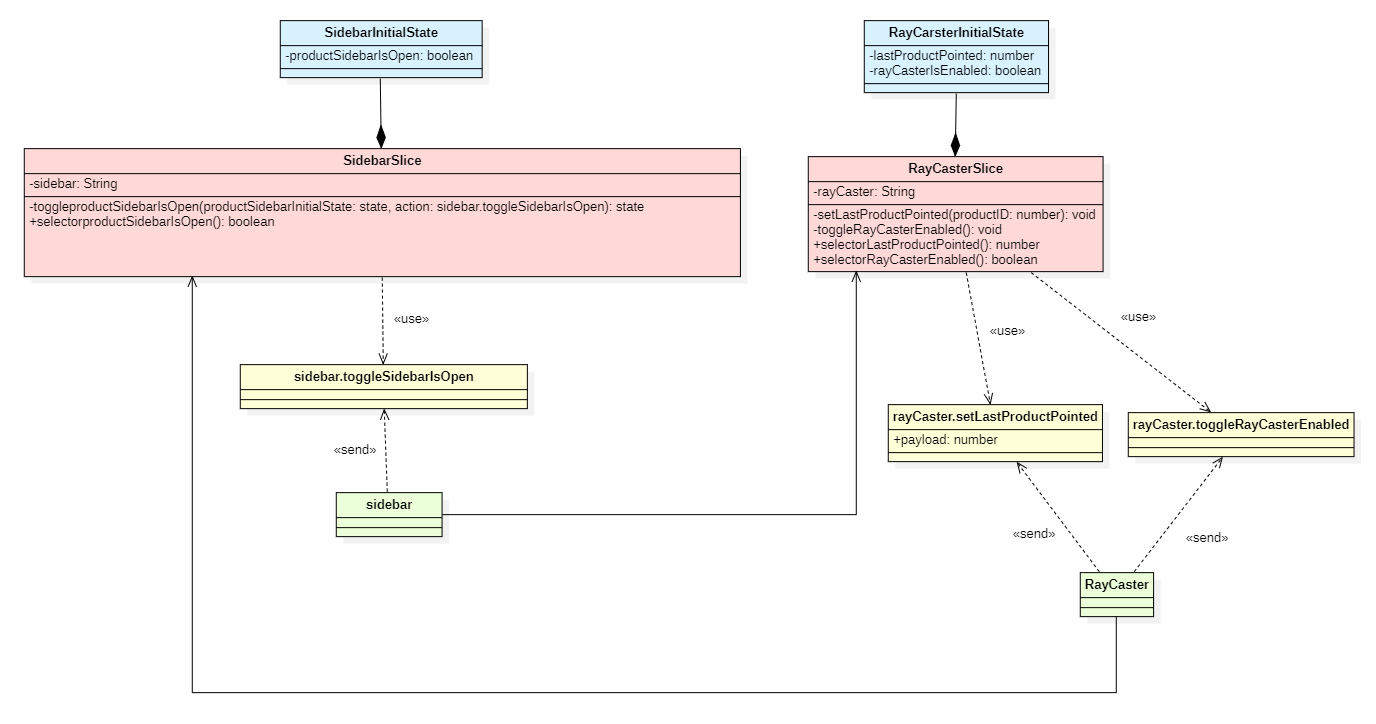
\includegraphics[scale=0.75, keepaspectratio]{./res/images/InterfaceFeaturesDiagram.PNG}
	\caption[UML delle classi InterfaceFeaturesDiagram]{
	UML delle classi InterfaceFeaturesDiagram.
	\\
	\textbf{Legenda}: 
	[\textit{Slices}: rosso] -
	[\textit{Actions}: giallo] -
	[\textit{Model classes}: grigio] -
	[\textit{Initial states}: azzurro] -
	[\textit{UI React components}: verde]}
\end{figure}
\end{landscape}
\restoregeometry
\paragraph*{Descrizione del diagramma:}
InterfaceFeaturesDiagram include i componenti necessari per il corretto aggiornamento dell'interfaccia utente.
\begin{itemize}
		\item \textbf{SidebarSlice}
		\\\\
		\textbf{Dipendenze}:
		\begin{itemize}
			\item \textit{SidebarInitialState} (Composizione): si occupa della costruzione e distruzione dell'istanza di SidebarInitialState
			che non viene condivisa con altri componenti in quanto SidebarSlice si occupa in modo esclusivo della sua gestione.
			\item \textit{sidebar.toggleSidebarIsOpen} (Dipendenza semplice \textless use\textgreater): cattura un'istanza di sidebar.toggleSidebarIsOpen
			per commutare il valore dell'attributo productSidebarIsOpen in SidebarInitialState.
		\end{itemize}
		\textbf{Actions catturate}:
		\begin{itemize}
			\item \textit{sidebar.toggleSidebarIsOpen}: utilizzata dal reducer per chiamare \textit{toggleSidebarIsOpen}.
		\end{itemize}
		\item \textbf{SideBar}
		\\\\
		\textbf{Dipendenze}:
		\begin{itemize}
			\item \textit{RayCasterSlice} (Associazione): utilizza selectorLastProductPointed per ricavare l'ID dell'ultimo 
			prodotto puntato dal rayCaster. Se il raycaster non sta puntando a nessun prodotto il selettore ritorna null.
			\item \textit{sidebar.toggleSidebarIsOpen} (Dipendenza semplice \textless send\textgreater): emette un'azione
			sidebar.toggleSidebarIsOpen.
		\end{itemize}
		\textbf{Action emesse}:
		\begin{itemize}
			\item \textit{sidebar.toggleSidebarIsOpen}: emessa quando l'utente apre o chiude la sidebar
		\end{itemize}
		\item \textbf{RayCasterSlice}
		\\\\
		\textbf{Dipendenze}:
		\begin{itemize}
			\item \textit{RayCarsterInitialState} (Composizione): si occupa della costruzione e distruzione dell'istanza di RayCarsterInitialState
			che non viene condivisa con altri componenti in quanto RayCasterSlice si occupa in modo esclusivo della sua gestione.
			\item \textit{rayCaster.setLastProductPointed} (Dipendenza semplice \textless use\textgreater): cattura un'istanza di rayCaster.setLastProductPointed
			per aggiornare il valore dell'attributo lastProductPointed con l'ID dell'ultimo oggetto puntato dal raycaster. 
			\item \textit{rayCaster.toggleRayCasterEnabled} (Dipendenza semplice \textless use\textgreater): cattura un'istanza di sidebar.toggleSidebarIsOpen
			per commutare il valore dell'attributo rayCasterIsEnabled in SidebarInitialState. 
		\end{itemize}
		\textbf{Action catturate}:
		\begin{itemize}
			\item \textit{rayCaster.setLastProductPointed}: utilizzata dal reducer per chiamare \textit{setLastProductPointed}.
			\item \textit{rayCaster.toggleRayCasterEnabled}: utilizzata dal reducer per chiamare \textit{toggleRayCasterEnabled}.
		\end{itemize}
		\item \textbf{RayCaster}
		\\\\
		\textbf{Dipendenze}:
		\begin{itemize}
			\item \textit{SidebarSlice} (Associazione): utilizza selectorproductSidebarIsOpen.
			\item \textit{rayCaster.setLastProductPointed} (Dipendenza semplice \textless send\textgreater): emette un'azione
			rayCaster.setLastProductPointed.
			\item \textit{rayCaster.toggleRayCasterEnabled} (Dipendenza semplice \textless send\textgreater): emette un'azione
			rayCaster.toggleRayCasterEnabled.
		\end{itemize}
		\textbf{Interazioni}:
		\begin{itemize}
			\item \textit{SidebarSlice}: chiama selectorproductSidebarIsOpen per verificare se la sidebar
			è aperta o chiusa in modo da abilitare o disabilitare il raycaster a seconda del caso.
		\end{itemize}
		\textbf{Action emesse}:
		\begin{itemize}
			\item \textit{rayCaster.setLastProductPointed}: emessa quando il raycaster punta un prodotto all'interno dell'ambiente 3D.
			\item \textit{rayCaster.toggleRayCasterEnabled}: emessa quando viene aperta la sidebar per disabilitare i raycaster.
		\end{itemize}
\end{itemize}


\newgeometry{margin=0.5cm}
\begin{landscape}
\thispagestyle{empty}
\subsubsection{StoreDiagram}
\begin{figure}[H]
	\centering
	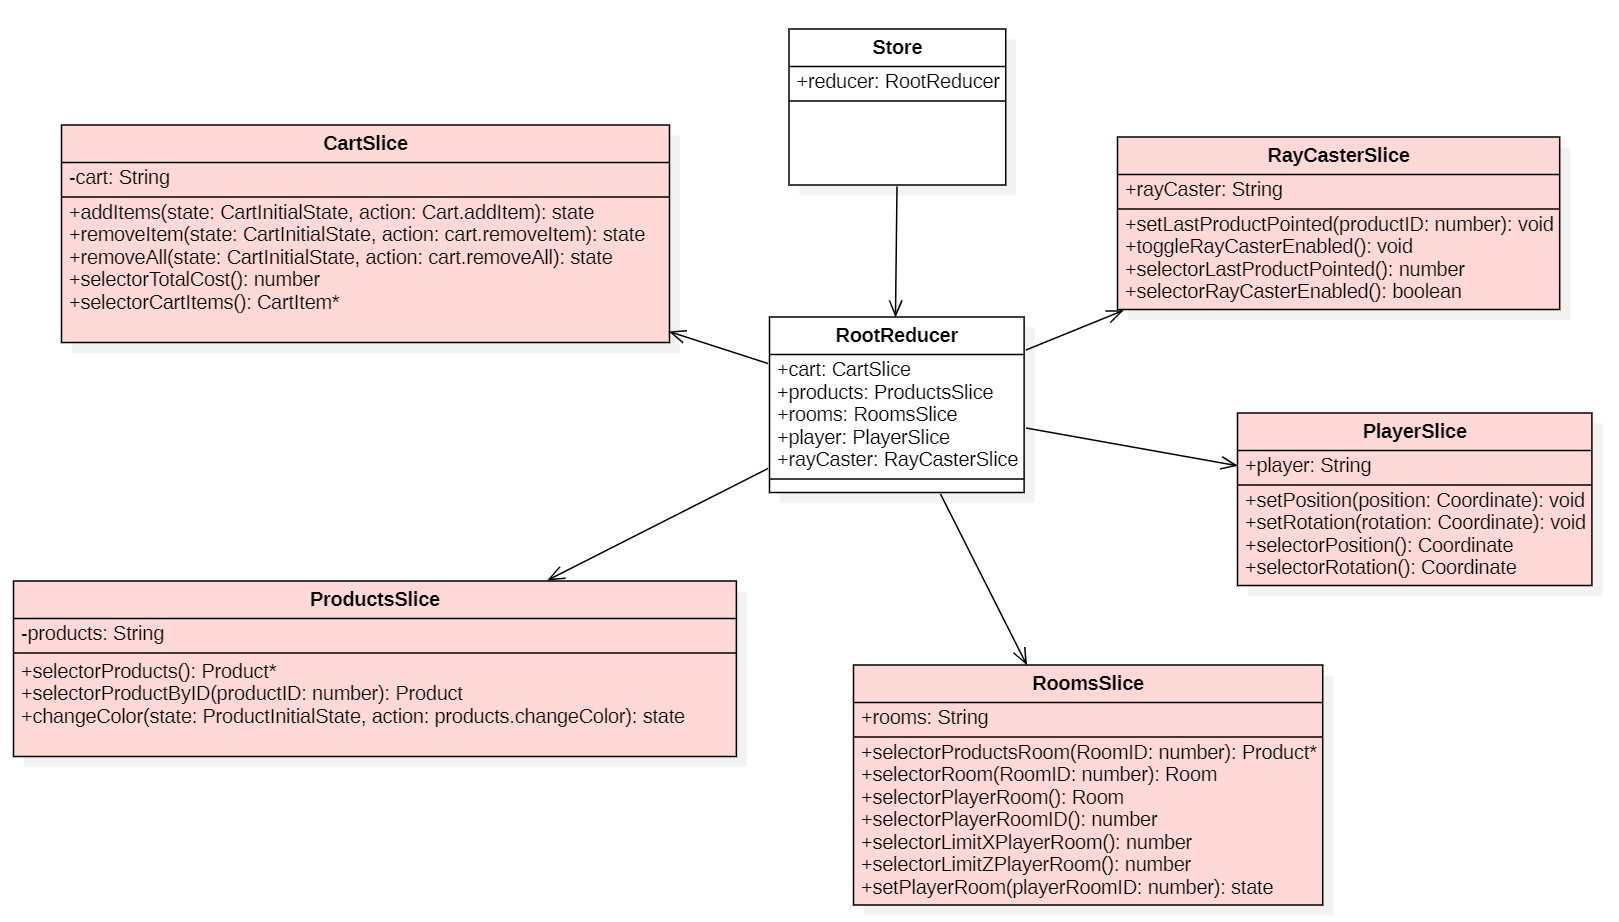
\includegraphics[scale=0.7, keepaspectratio]{./res/images/StoreDiagram.PNG}
	\caption[UML delle classi StoreDiagram]{
	UML delle classi StoreDiagram.
	\\
	\textbf{Legenda}: 
	[\textit{Slices}: rosso] -
	[\textit{Model classes}: grigio] -
	[\textit{Initial states}: azzurro]}
\end{figure}
\end{landscape}
\restoregeometry
\paragraph*{Descrizione del diagramma:}
Include lo \textit{store} e le slice che compongono lo stato globale dell'applicazione.
\begin{itemize}
		\item \textbf{Store}
		\\\\
		\textbf{Dipendenze}:
		\begin{itemize}
			\item \textit{RootReducer} (Associazione): ha un attributo RootReducer che permette di combinare piú slice con cui lo store interagisce 
			per modificare lo stato globale dell'applicazione.
		\end{itemize}
		\item \textbf{RootReducer}
		\\\\
		\textbf{Dipendenze}:
		\begin{itemize}
			\item \textit{CartSlice} (Associazione): ha un attributo CartSlice per offrire allo store l'accesso alla slice.
			\item \textit{ProductsSlice} (Associazione): ha un attributo ProductsSlice per offrire allo store l'accesso alla slice.
			\item \textit{DecorationsSlice} (Associazione): ha un attributo DecorationsSlice per offrire allo store l'accesso alla slice.
			\item \textit{SidebarSlice} (Associazione): ha un attributo SidebarSlice per offrire allo store l'accesso alla slice.
			\item \textit{PlayerSlice} (Associazione): ha un attributo PlayerSlice per offrire allo store l'accesso alla slice.
			\item \textit{RayCasterSlice} (Associazione): ha un attributo RayCasterSlice per offrire allo store l'accesso alla slice.
		\end{itemize}
		\item \textbf{DecorationsSlice}
		\\\\
		\textbf{Dipendenze}:
		\begin{itemize}
			\item \textit{DecorationInitialState}: si occupa della costruzione e distruzione dell'istanza di DecorationInitialState
			che non viene condivisa con altri componenti in quanto DecorationsSlice si occupa in modo esclusivo della sua gestione.
		\end{itemize}

		\item \textbf{DecorationInitialState}
		\\\\
		\textbf{Dipendenze}:
		\begin{itemize}
			\item \textit{Decoration}: contiene la lista delle decorazioni presenti all'interno dell'ambiente 3D.
		\end{itemize}

		\item \textbf{Decoration}
		\\\\
		\textbf{Dipendenze}:
		\begin{itemize}
			\item \textit{DecorationModelGLTF} (Composizione): costruisce l'istanza del modello che rappresenta la decorazione.
		\end{itemize}
\end{itemize}

\subsubsection{SkyLevelReactComponentsHierarchy}
\begin{figure}[H]
	\centering
	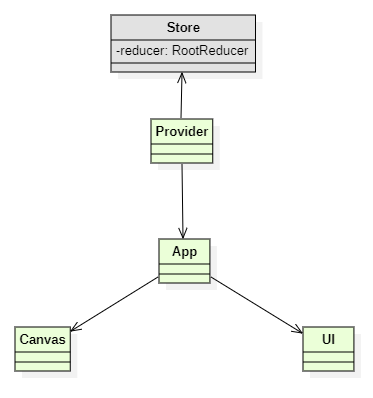
\includegraphics[scale=0.75, keepaspectratio]{./res/images/SkyLevelReactComponentHierarchy.PNG}
	\caption[UML delle classi SkyLevelReactComponentsHierarchy]{
	UML delle classi SkyLevelReactComponentsHierarchy.
	\\
	\textbf{Legenda}: 
	[\textit{Slices}: rosso] -
	[\textit{Actions}: giallo] -
	[\textit{Model classes}: grigio] -
	[\textit{Initial states}: azzurro] -
	[\textit{UI React components}: verde]}
\end{figure}

\paragraph*{Descrizione del diagramma:}
Include i macrocomponenti React che costituiscono l'applicazione.
\begin{itemize}
		\item \textbf{Provider}
		\\\\
		\textbf{Dipendenze}:
		\begin{itemize}
			\item \textit{Store} (Associazione): tutti i componenti figli fanno riferimento allo store passato come props al 
			componente Provider.
			\item \textit{App} (Associazione): contiene i componenti che costituiscono l'applicazione che comunicano con lo store.
		\end{itemize}

		\item \textbf{App}
		\\\\
		\textbf{Dipendenze}:
		\begin{itemize}
			\item \textit{IU} (Composizione): crea il componente figlio che contiene l'interfaccia utente.
			\item \textit{Canvas} (Coomposizione): crea il componente figlio che contiene l'ambiente 3D.
		\end{itemize}
\end{itemize}

		
\newgeometry{margin=0.5cm}
\begin{landscape}
\thispagestyle{empty}
\subsubsection{UIReactComponentsHierarchy}
\begin{figure}[H]
	\centering
	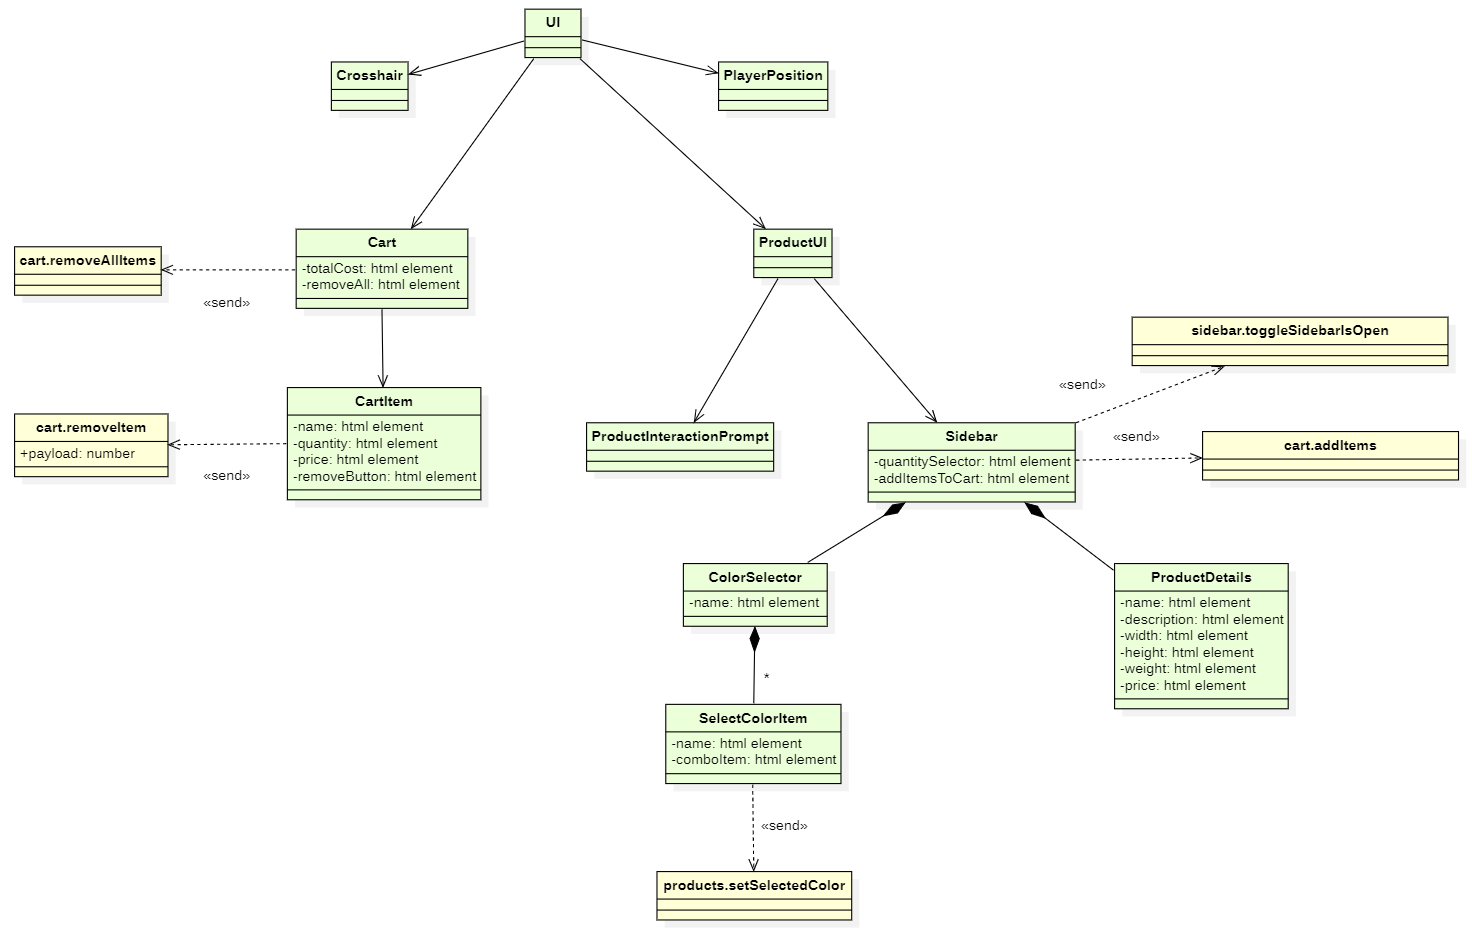
\includegraphics[scale=0.7, keepaspectratio]{./res/images/UIReactComponentsHierarchy.PNG}
	\caption[UML delle classi UIReactComponentsHierarchy]{
	UML delle classi UIReactComponentsHierarchy.
	\\
	\textbf{Legenda}: 
	[\textit{Slices}: rosso] -
	[\textit{Actions}: giallo] -
	[\textit{Model classes}: grigio] -
	[\textit{Initial states}: azzurro] -
	[\textit{UI React components}: verde]}
\end{figure}
\end{landscape}
\restoregeometry
\paragraph*{Descrizione del diagramma:}
Contiene i componenti che costituiscono l'interfaccia utente.
Lo schema illustra come è organizzato l'albero delle discendenze tra componenti dell'interfaccia utente.
Le dipendenze di composizione di un componente indicano che il gestisce il ciclo di vita dei componenti figli che sono contenuti 
al suo interno.

\newgeometry{margin=0.5cm}
\begin{landscape}
\thispagestyle{empty}
\subsubsection{CanvasReactComponentsHierarchy}
\begin{figure}[H]
	\centering
	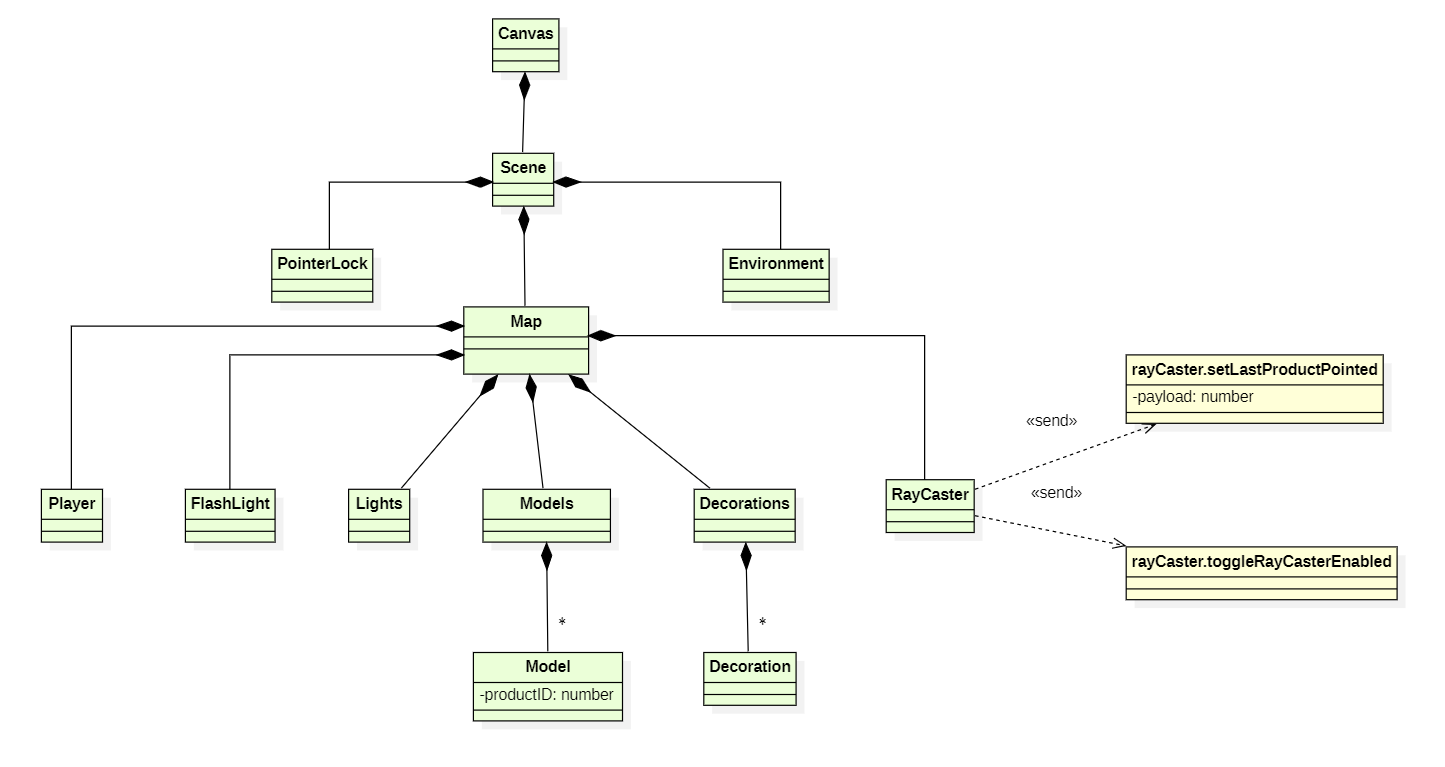
\includegraphics[scale=0.7 , keepaspectratio]{./res/images/CanvasReactComponentsHierarchy.PNG}
	\caption[UML delle classi CanvasReactComponentsHierarchy]{
	UML delle classi CanvasReactComponentsHierarchy.
	\\
	\textbf{Legenda}: 
	[\textit{Slices}: rosso] -
	[\textit{Actions}: giallo] -
	[\textit{Model classes}: grigio] -
	[\textit{Initial states}: azzurro] -
	[\textit{UI React components}: verde]}
\end{figure}
\end{landscape}
\restoregeometry

\paragraph*{Descrizione del diagramma:}
Contiene i componenti che costituiscono l'ambiente 3D.
Lo schema illustra come è organizzato l'albero delle discendenze tra componenti del canvas.
Le dipendenze di composizione di un componente indicano che il gestisce il ciclo di vita dei componenti figli che sono contenuti 
al suo interno.

\subsection{Architettura di deployment}

come viene fatta la build e come viene configurato il server che ospita l'app

\subsection{Altri aspetti di design}
























